%----------------------------------------------------------------------------------------
%	PACKAGES AND OTHER DOCUMENT CONFIGURATIONS
%----------------------------------------------------------------------------------------

\documentclass[a4paper,10pt]{article} % Paper size, default font size and one-sided paper
\usepackage{geometry}
\geometry{tmargin=25mm,bmargin=25mm,lmargin=25mm,rmargin=20mm}

\usepackage{amsmath}    		% Additional math functionality
\usepackage{amssymb}    		% Additional math functionality
\usepackage{ifpdf}
\usepackage[final]{pdfpages}
\usepackage{setspace}
\usepackage{afterpage}
\usepackage{titlesec}
\usepackage{fancyhdr}
\usepackage{listings}
\usepackage{xcolor}
\usepackage[english]{babel}
\usepackage{hyperref}
\usepackage[latin1]{inputenc}
\usepackage{tikz}
\usetikzlibrary{shapes,arrows}
\usepackage{cleveref}

%setup url
\hypersetup{
    colorlinks=true,       % false: boxed links; true: colored links
    urlcolor  = blue,           % color of external links
    linkcolor = black
}

%setup header
\pagestyle{fancy}
\fancyhf{}
\fancyhead[LE,RO]{Pascal Buholzer, Fabio Dubois, Miro Voellmy, Milan Schilling}
\fancyhead[RE,LO]{Vision Algorithms for Mobile Robotics}
%\fancyfoot[CE,CO]{\leftmark}
\fancyfoot[LE,RO]{\thepage}

%setup code
\lstset{
  language=C,               	  % choose the language of the code
  numbers=left,                   % where to put the line-numbers
  stepnumber=1,                   % the step between two line-numbers.        
  numbersep=5pt,                  % how far the line-numbers are from the code
  backgroundcolor=\color{white},  % choose the background color. You must add \usepackage{color}
  showspaces=false,               % show spaces adding particular underscores
  showstringspaces=false,         % underline spaces within strings
  showtabs=false,                 % show tabs within strings adding particular underscores
  tabsize=2,                      % sets default tabsize to 2 spaces
  captionpos=b,                   % sets the caption-position to bottom
  breaklines=true,                % sets automatic line breaking
  breakatwhitespace=true,         % sets if automatic breaks should only happen at whitespace
  title=\lstname,                 % show the filename of files included with \lstinputlisting;
}

%setup file input directory
\makeatletter
\def\input@path{{./includes/}}
\makeatother

%setup graphics directory
\graphicspath{{./graphics/}}


%%%%%%%%%%%%%%%%%%%%%%%%%%%%%%%%%%%%%%%%%%%%%%%%%%%%%%%%%%%%%%%%%%%%%%%%%%%%%%%%%%
\begin{document}

\title{Visual Odometry Pipeline}
\author{Pascal Buholzer, Fabio Dubois, Milan Schilling, Miro Voellmy}
\maketitle

% Table of Contents depth (TODO change if necessary)
\newpage
\section*{Symbols}
\newpage


\tableofcontents
\newpage
\section{Introduction}
The aim of this mini project is the development of a visual odometry pipeline. This pipeline takes the consecutive gray-scale images of a single digital camera as input. Therefore the pipeline developed in this mini project is a monocular visual odometry pipeline.

The output of the pipeline is the position of the camera in relation to its initial position for each frame.



keywords:
(VO, sequential, monocular, markov assumption)
\newpage
\section{Implementation}

\subsection{Framework}
This pipeline was developed in MATLAB. Since the group consists of four students, a Git repository was used to be able to work on different files simultaneously, and to enable version control.
(keywords: MATLAB, Git)

\subsubsection{Coordinate Frames}
In this mini project the coordinate frames were defined as shown in \cref{img_coord_frames}. The camera coordinates are in a way oriented, that the x-y plane lies parallel to the image plane, while the z-axis is pointing towards the scenery. The world frame however is oriented in such a way that the x-y plane is parallel to the ground and the the z-axis is pointing upwards.

The origin of the world frame is at the same location as the origin of the first boot-strap image.

\begin{figure}[ht]
	\centering
	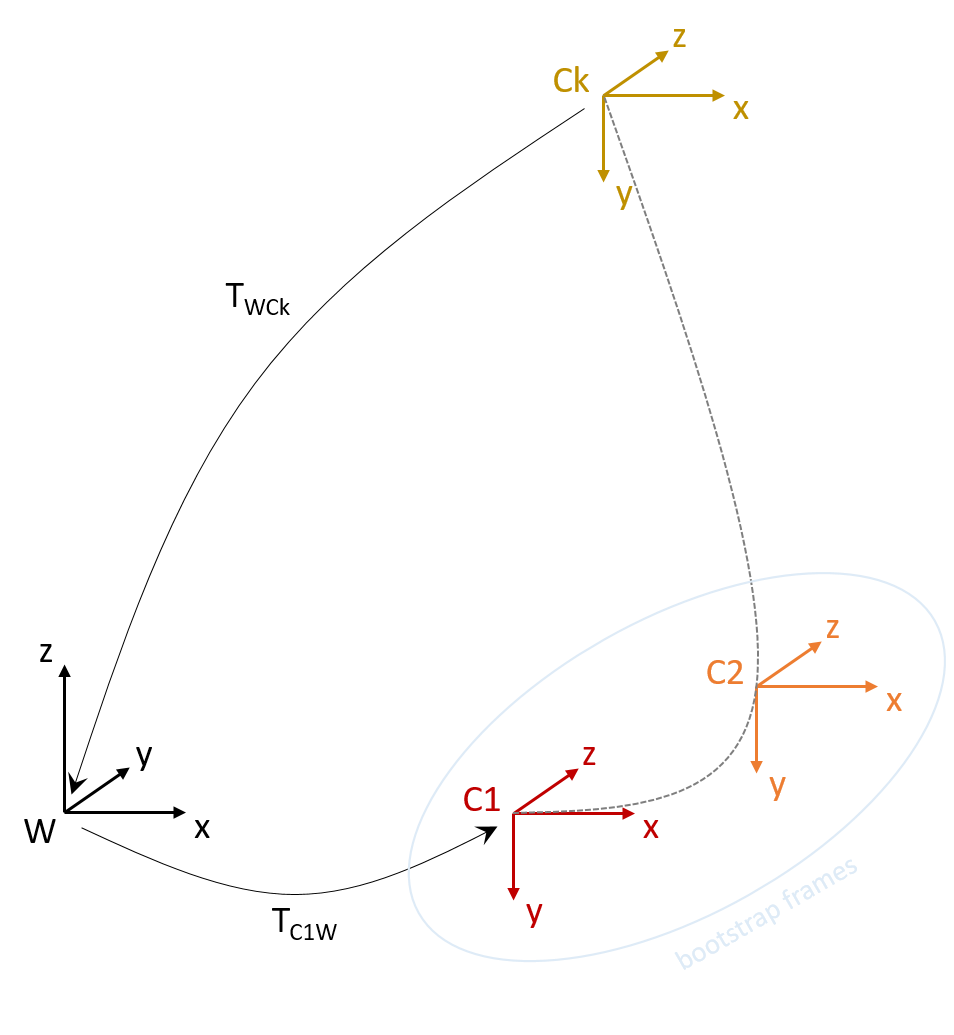
\includegraphics[width=0.5\textwidth]{coord_frames}
	\caption{Coordinate Frames}
	\label{img_coord_frames}
\end{figure}

\subsubsection{Pipeline overview}

As shown in \cref{img_flow_rough} the pipeline consists mainly of three parts, a bootstrap, the initialisation and the continuous operation. In \cref{sec_init} and \cref{sec_cont_op} the initialisation and the continuous operation are described in detail.

\begin{figure}[ht]
	\centering
	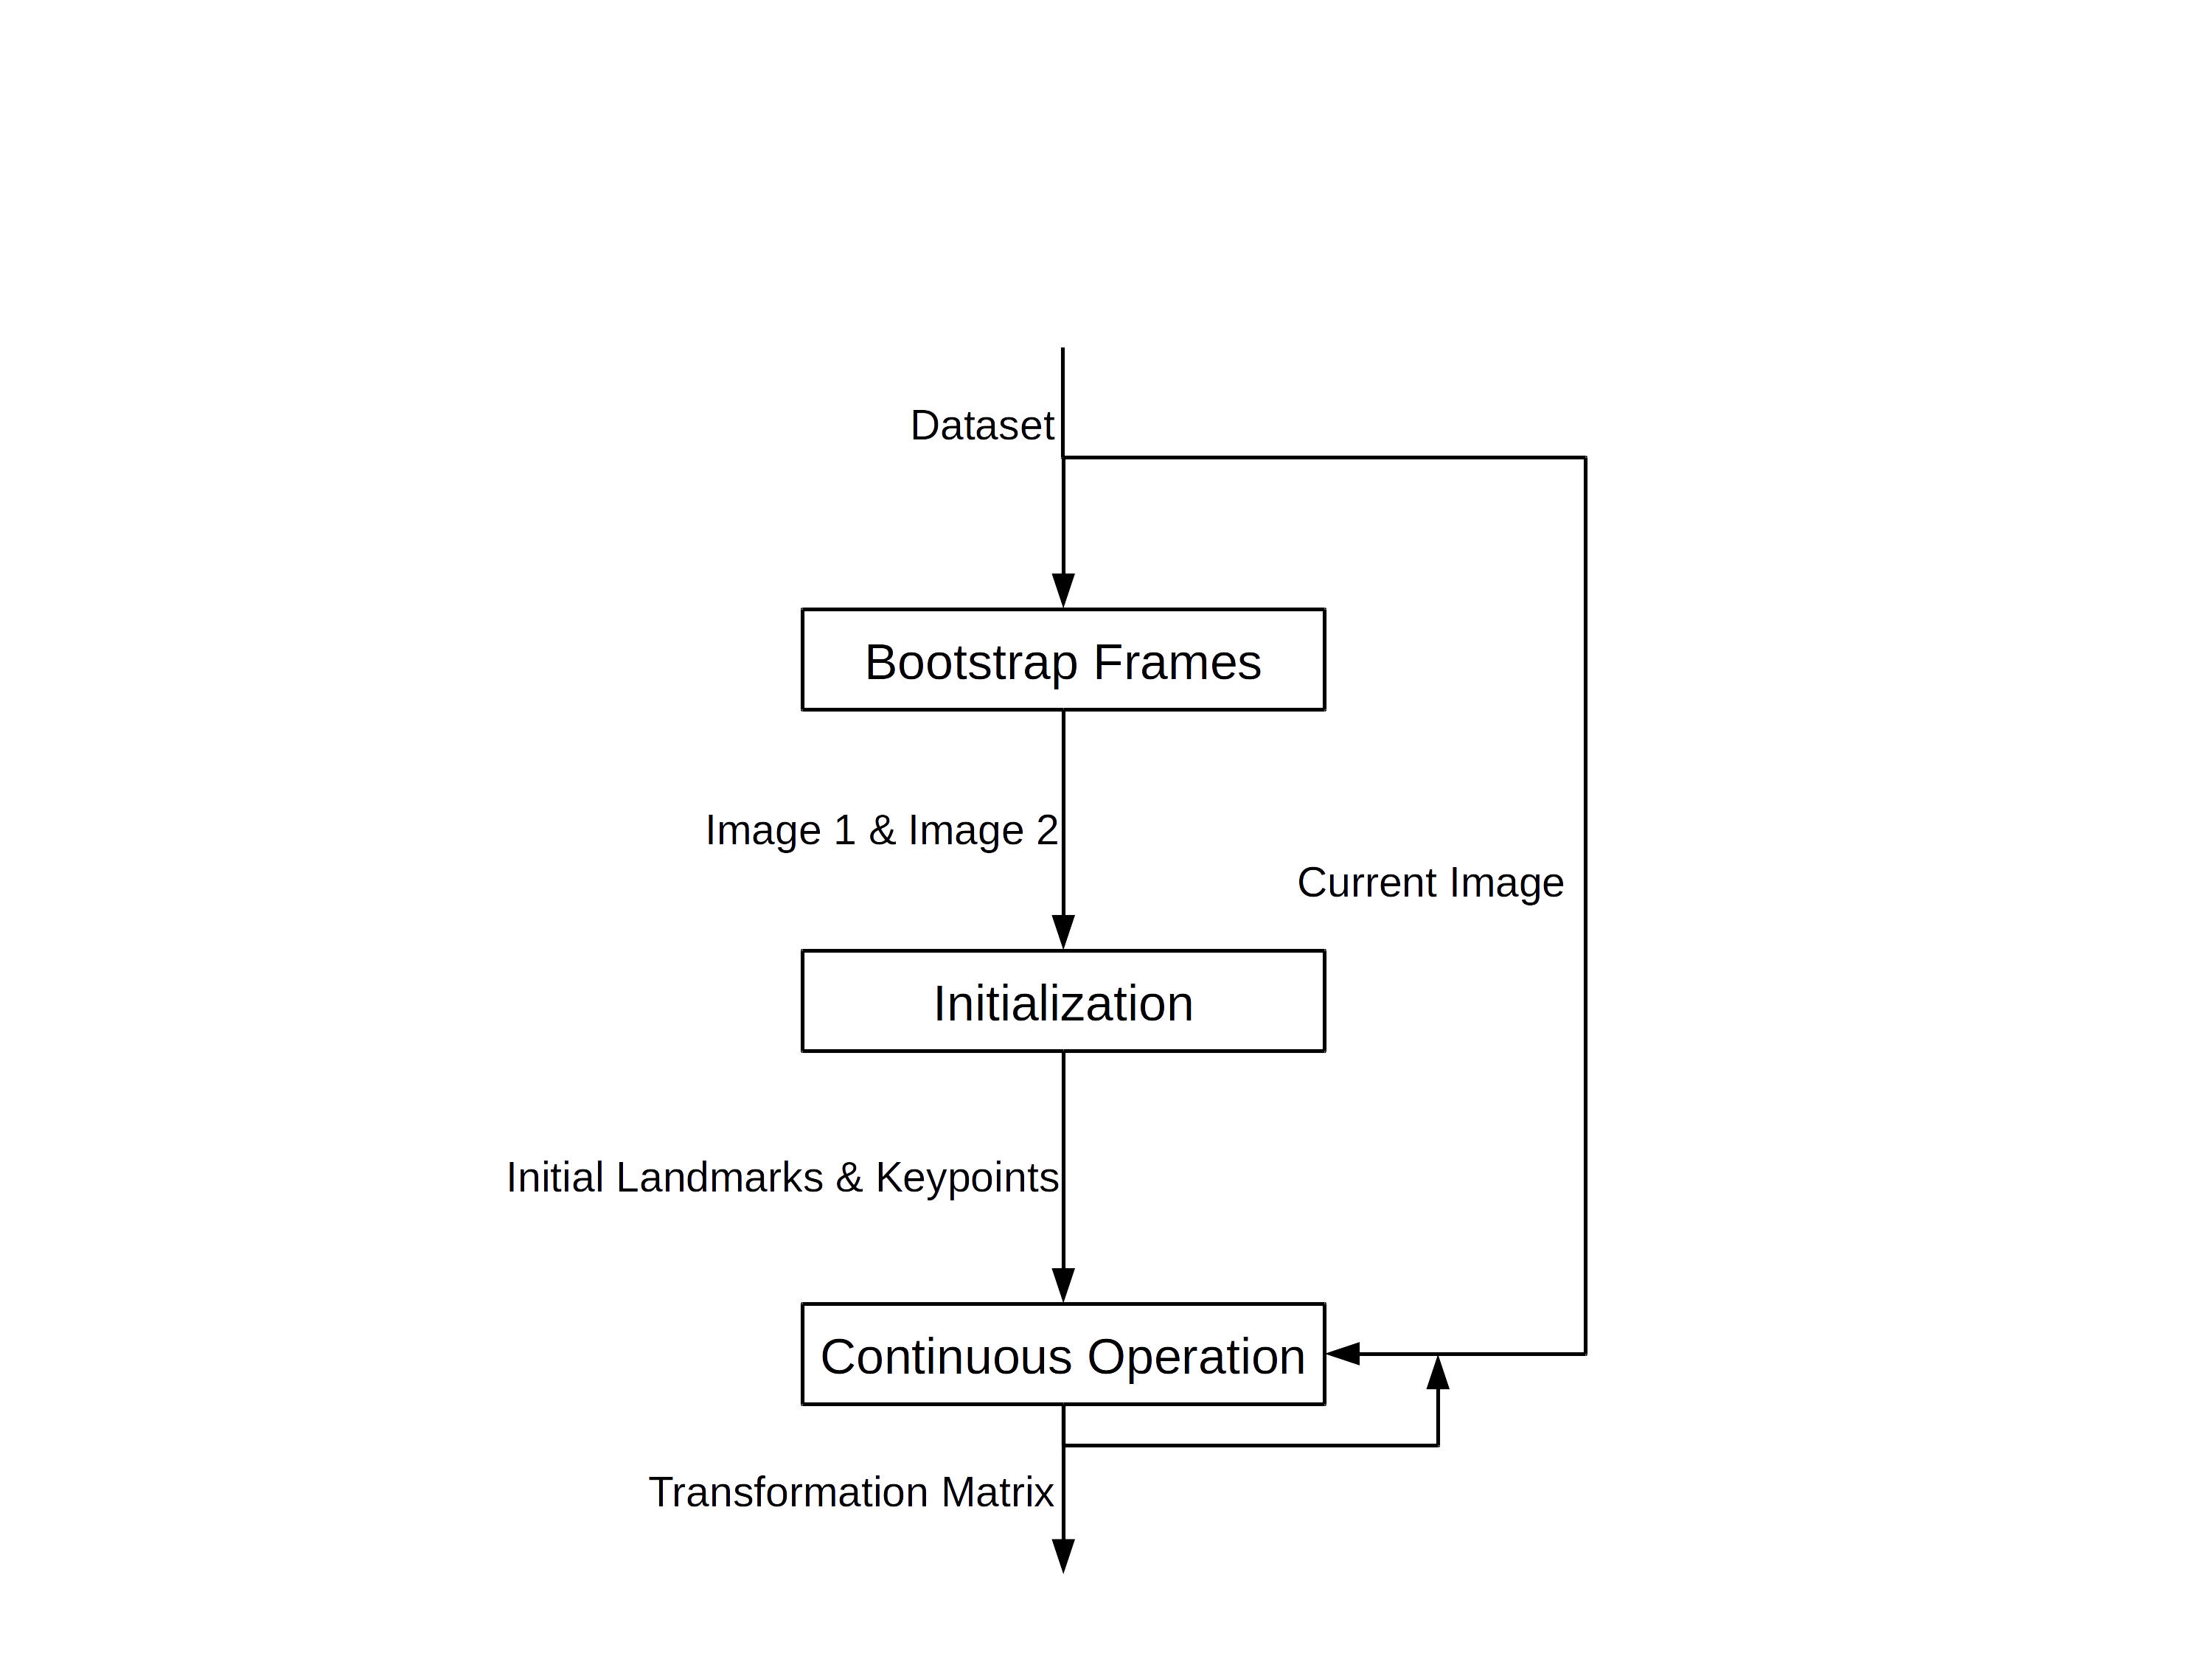
\includegraphics[width=0.8\textwidth]{rough_flow}
	\caption{Rough Flow chart}
	\label{img_flow_rough}
\end{figure}
%\input{pipeline_overview}
\subsubsection{Options and parameters}
(keywords: parameter handling, GUI)


\subsection{Initialization}
\label{sec_init}


\begin{figure}[ht]
	\centering
	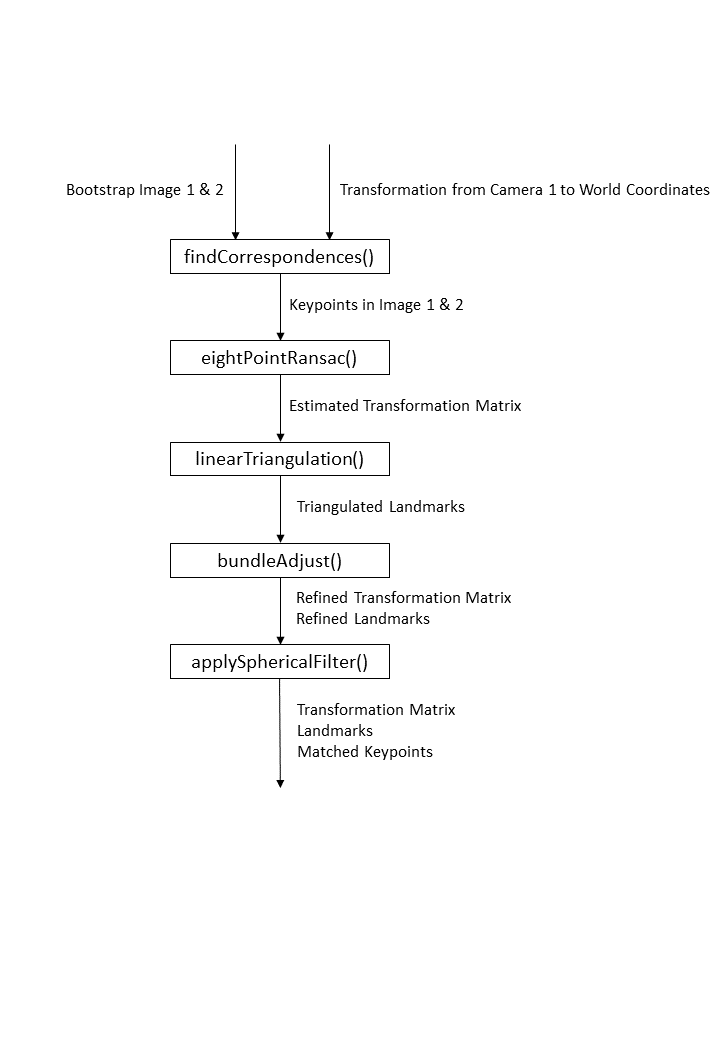
\includegraphics[width=0.8\textwidth]{init_chart}
	\caption{Init Flow chart}
	\label{img_flow_init}
\end{figure}
\clearpage{\pagestyle{plain}\cleardoublepage}
\subsection{Continuous Operation}
\label{sec_cont_op}


\begin{figure}[ht]
	\centering
	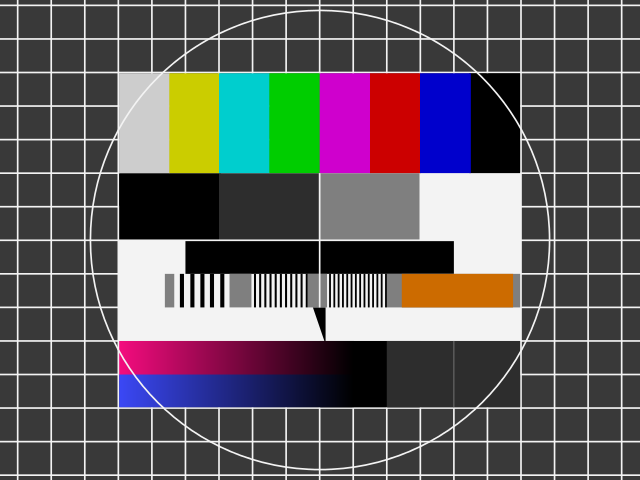
\includegraphics[width=0.8\textwidth]{test}
	\caption{Cont Flow chart}
	\label{img_flow_cont}
\end{figure}
\clearpage{\pagestyle{plain}\cleardoublepage}
\newpage
\section{Results}

\subsection{Overall performance}
(keywords: Real time ness, comparison to groundtruth, compare different datasets
Impact of features)
\newpage
\section{Discussion}
What have we learned, what worked?

Possible future work, improvements (loop closure, ...)

\section{Conclusion}

\newpage
%\subsection*{code.m}
%\lstinputlisting[language=C]{../code/lab06/lab06.ino}

\end{document}